\chapter{The Digital Twin Breathes}
\label{ch:twin}

\section{What was built}

Isaac Sim 5.1 now simulates the UR5e under PhysX, and ROS~2 commands it: an OmniGraph action
graph publishes the simulated encoders at 60\,Hz (\texttt{/joint\_states}, measured 59.99\,Hz,
$\sigma{=}0.9$\,ms) and feeds subscribed \texttt{JointState} commands into an Articulation
Controller. A hand-published message from a terminal moved the simulated arm. The digital twin
of chapter~\ref{ch:why} stopped being a diagram on 5~July~2026.

\begin{figure}[h]\centering
  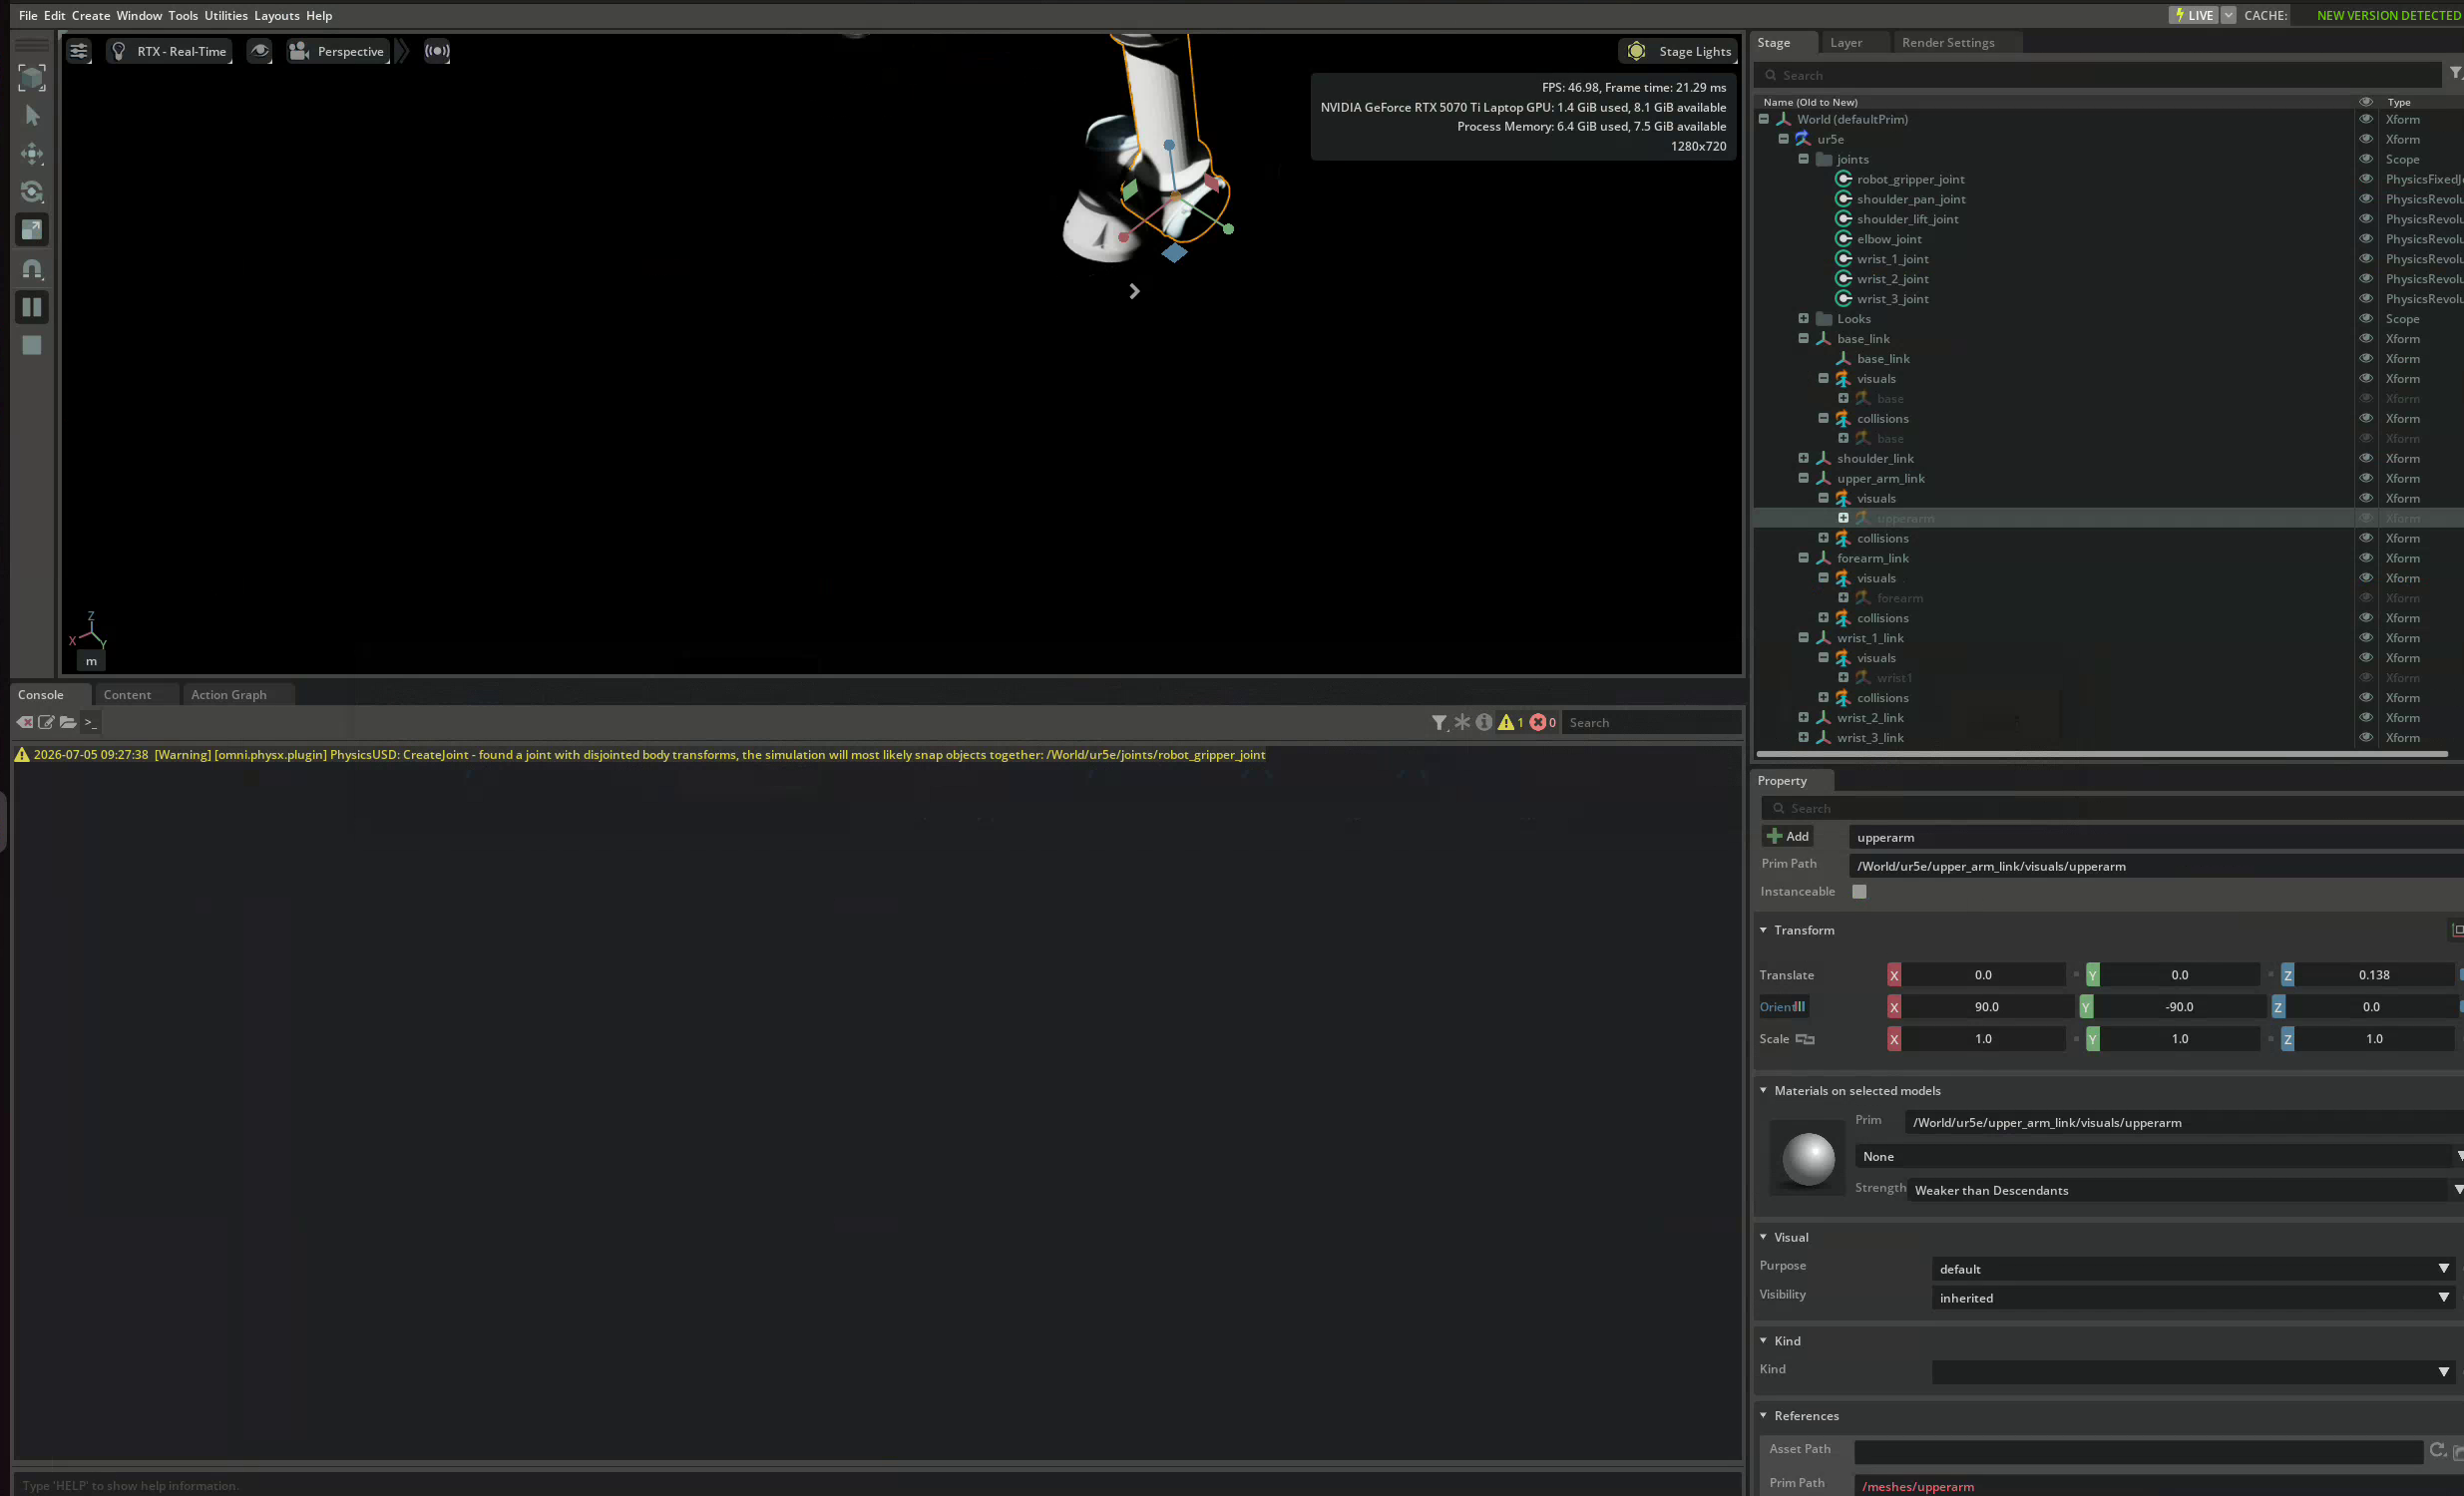
\includegraphics[width=0.95\linewidth]{figures/ch04_isaac_first_command.png}
  \caption{First ROS-commanded motion in Isaac Sim: the UR5e mid-sweep after a
  \texttt{JointState} message published from the host terminal. Right: the asset's true
  structure in the Stage tree --- links, joints scope, and the \texttt{root\_joint} that
  turned out to carry the Articulation Root.}
\end{figure}

The graph is five nodes: \emph{On Playback Tick} drives \emph{ROS2 Publish Joint State},
\emph{ROS2 Subscribe JointState} $\to$ \emph{Articulation Controller}, with \emph{Read
Simulation Time} stamping headers. The stage lives in the repo
(\texttt{ros2\_ws/isaac/VanguardArm.usd}); a bonus discovery in its tree: the 5.1 UR5e asset
ships \emph{with a gripper} (\texttt{Gripper} prim + \texttt{robot\_gripper\_joint}), so
grasping work gets simulated fingers for free.

\section{The debugging ledger (four traps, all now labeled)}

\begin{lesson}
\textbf{\texttt{omniverse:///} is a server you don't have.} Save As defaults to a Nucleus URL;
a bare filename typed there fails with \emph{``Cannot save layer... Error: Connection''} — and
took the whole action graph with it the first night (unsaved stage, Isaac closed). Rule: in
any Omniverse file dialog, click \emph{My Computer} and verify the path bar shows a local path
\emph{before} naming the file. Corollary: save the stage before building anything on it.
\end{lesson}

\begin{lesson}
\textbf{USD prim paths are case-sensitive.} Graph nodes targeting \texttt{/World/ur5e} while
the prim differed only in case produced hundreds of \emph{Failed to find articulation} errors
— and an empty ROS topic list that masqueraded as a DDS problem. Debugging order adopted:
read the prim path from the Stage panel and set targets with the eyedropper, never by typing.
\end{lesson}

\begin{lesson}
\textbf{errno 28 lies.} Thousands of \emph{``No space left on device''} errors at startup with
255\,GB free: inotify \emph{watch-limit} exhaustion (\texttt{fs.inotify.max\_user\_watches},
default 65{,}536 — Isaac watches every extension directory). Fixed permanently via sysctl
(1M watches). The error string reports ENOSPC; the device that is ``full'' is a kernel table,
not the disk.
\end{lesson}

\begin{lesson}
\textbf{The Articulation Root is not where you point.} With the path case fixed, physics still
found no articulation: on fixed-base Isaac assets the \texttt{ArticulationRootAPI} sits on the
\emph{fixed base joint} (\texttt{/World/ur5e/root\_joint}), not the robot's outer Xform. Both
ROS nodes had to target the root joint. General rule: target the prim that \emph{carries the
API}, findable by clicking through the Stage tree and watching the Property panel for the
``Articulation Root'' section.
\end{lesson}

\section{Architecture note: why this layer stays thin}

The action graph deliberately does \emph{not} implement control: it is a transport shim ---
encoders out, position targets in. Control authority stays in \texttt{ros2\_control}, which
next connects to these topics via a \texttt{topic\_based} hardware interface so that the
\emph{identical} controller stack (and \texttt{send\_trajectory.py}, unmodified) runs against
Isaac exactly as it ran against mock hardware. One contract, three bottoms: mock, Isaac,
and --- in September --- motors. The topics are being renamed \texttt{/isaac\_joint\_states}
and \texttt{/isaac\_joint\_commands} accordingly, because the plain \texttt{/joint\_states}
name belongs to \texttt{ros2\_control}'s broadcaster in that stack.
